\section{Evaluation and Discussion}
\label{sec:ch3:results}

In this section, we qualitatively evaluate our algorithm, we describe our dataset of infeasible quadrotor camera trajectories and the experiments we conducted to quantitatively evaluate our algorithm, and we discuss our key results.

In the experiments in this section, we evaluate our algorithm, a modified version of our algorithm where we update $\bar{\dot{s}}$ for 50 iterations (instead of our usual 10 iterations), and a spacetime constraints approach.
We describe the exact spacetime constraints problem formulation we use in our experiments in Section~\ref{sec:ch3:spacetime}.
We discretize each trajectory in our experiments at a moderate resolution of 100 time samples, unless otherwise noted.

\paragraph{Comparing Shot Previews and Real Video Footage}

In Figure~\ref{fig:ch3:real}, we show a side-by-side comparison of a \textsc{Google Earth} shot preview and real video footage from an aggressive trajectory generated using our algorithm.
To capture this video footage, we use the quadrotor hardware platform described in Chapter~\ref{sec:ch2}.

\paragraph{Qualitative Comparison with Spacetime Constraints}

%(although in practice, the commercially available solver we used in our experiments occasionally encountered numerical difficulties with the spacetime constraints formulation, preventing it from finding a feasible solution for several of the trajectories in our dataset).

In Figure~\ref{fig:ch3:easing}, we show progress curves generated by our algorithm and spacetime constraints for an aggressive infeasible trajectory.
We observe that the progress curves produced by both algorithms are very similar.
We note that our algorithm and spacetime constraints are solving slightly different problems, so we do not expect the solutions to be identical.
In Figure~\ref{fig:ch3:limits}, we show that our algorithm remains within the prescribed velocity and control force limits, when generating the output trajectory shown in Figure~\ref{fig:ch3:easing}.

%It is also worth noting that our algorithm and spacetime constraints are solving slightly different problems, so we do not expect the solutions to be identical.
%In particular, spacetime constraints is free to perturb the spatial layout of the trajectory. Again, this freedom is required in order to ensure that the spacetime constraints optimization problem is not over-constrained. 
%Having the freedom to perturb the spatial layout of trajectories can result in solutions that more closely adhere to the user's intended timing, at the expense of adhering less closely to the user's intended visual content.
%In contrast, our algorithm adheres to the user's intended visual content exactly, and therefore, can produce slightly larger perturbations of the user's intended timing.
%In Figure \ref{fig:easing}, we show progress curves generated by our algorithm and spacetime constraints.
%In particular, spacetime constraints is free to perturb the spatial layout of the trajectory. Again, this freedom is required in order to ensure that the spacetime constraints optimization problem is not over-constrained. 
%Having the freedom to perturb the spatial layout of trajectories can result in solutions that more closely adhere to the user's intended timing, at the expense of adhering less closely to the user's intended visual content.
%In contrast, our algorithm adheres to the user's intended visual content exactly, and therefore, can produce slightly larger perturbations of the user's intended timing.
%In Figure \ref{fig:easing}, we show progress curves generated by our algorithm and spacetime constraints.

%\paragraph{Comparing the Dimensionality of our Formulation with Spacetime Constraints}

%We briefly compare the dimensionality of our mathematical formulation to a spacetime constraints approach.
%At each time sample, spacetime constraints requires at least 6 scalar decision variables for the configuration of a quadrotor, and 4 scalar decision variables for the quadrotor control forces.
%In contrast, our formulation requires 5 scalar decision variables at each time sample.
%Both formulations lead to the same block bi-diagonal structure in the constraint Jacobian.
%Therefore, compared to spacetime constraints, our formulation reduces the required number of decision variables by at least 50\%, while preserving the efficient sparsity pattern in the constraint Jacobian.

\begin{figure*}[t]
\centering
\includegraphics[width=6.0in]{images/2016_siggraph/05_easing_curve_comparison.pdf}
\caption{
An aggressive infeasible trajectory (far left), the feasible output trajectory produced by our algorithm (near left), and the feasible progress curves produced by our algorithm and spacetime constraints for this trajectory (right).
As a baseline, we include the progress curve obtained by uniformly time stretching the input trajectory until it becomes feasible. Our algorithm and spacetime constraints produce similar progress curves, and both methods perturb the timing of the input trajectory much less than uniform time stretching.
}
\label{fig:ch3:easing}
\end{figure*}

\begin{figure*}[t!]
\centering
\includegraphics[width=6.0in]{images/2016_siggraph/06_easing_curve_comparison_3.pdf}
\caption{
Our algorithm perturbs the timing of the infeasible input trajectory shown in Figure~\ref{fig:ch3:easing} as little as possible, while remaining within our quadrotor's physical limits.
To demonstrate this behavior, we plot the infeasible input (top) and feasible output (bottom) progress curves, control force curves, and velocity curves.
For reference, we plot the infeasible input progress curve in grey underneath the feasible output progress curve.
We indicate control force and velocity limits  with horizontal dotted lines.
The feasible trajectory produced by our algorithm is at our quadrotor's physical limits for sustained periods, but never exceeds these physical limits.
}
\label{fig:ch3:limits}
\end{figure*}

\paragraph{Infeasible Trajectory Dataset}

\begin{figure*}[th!]
\centering
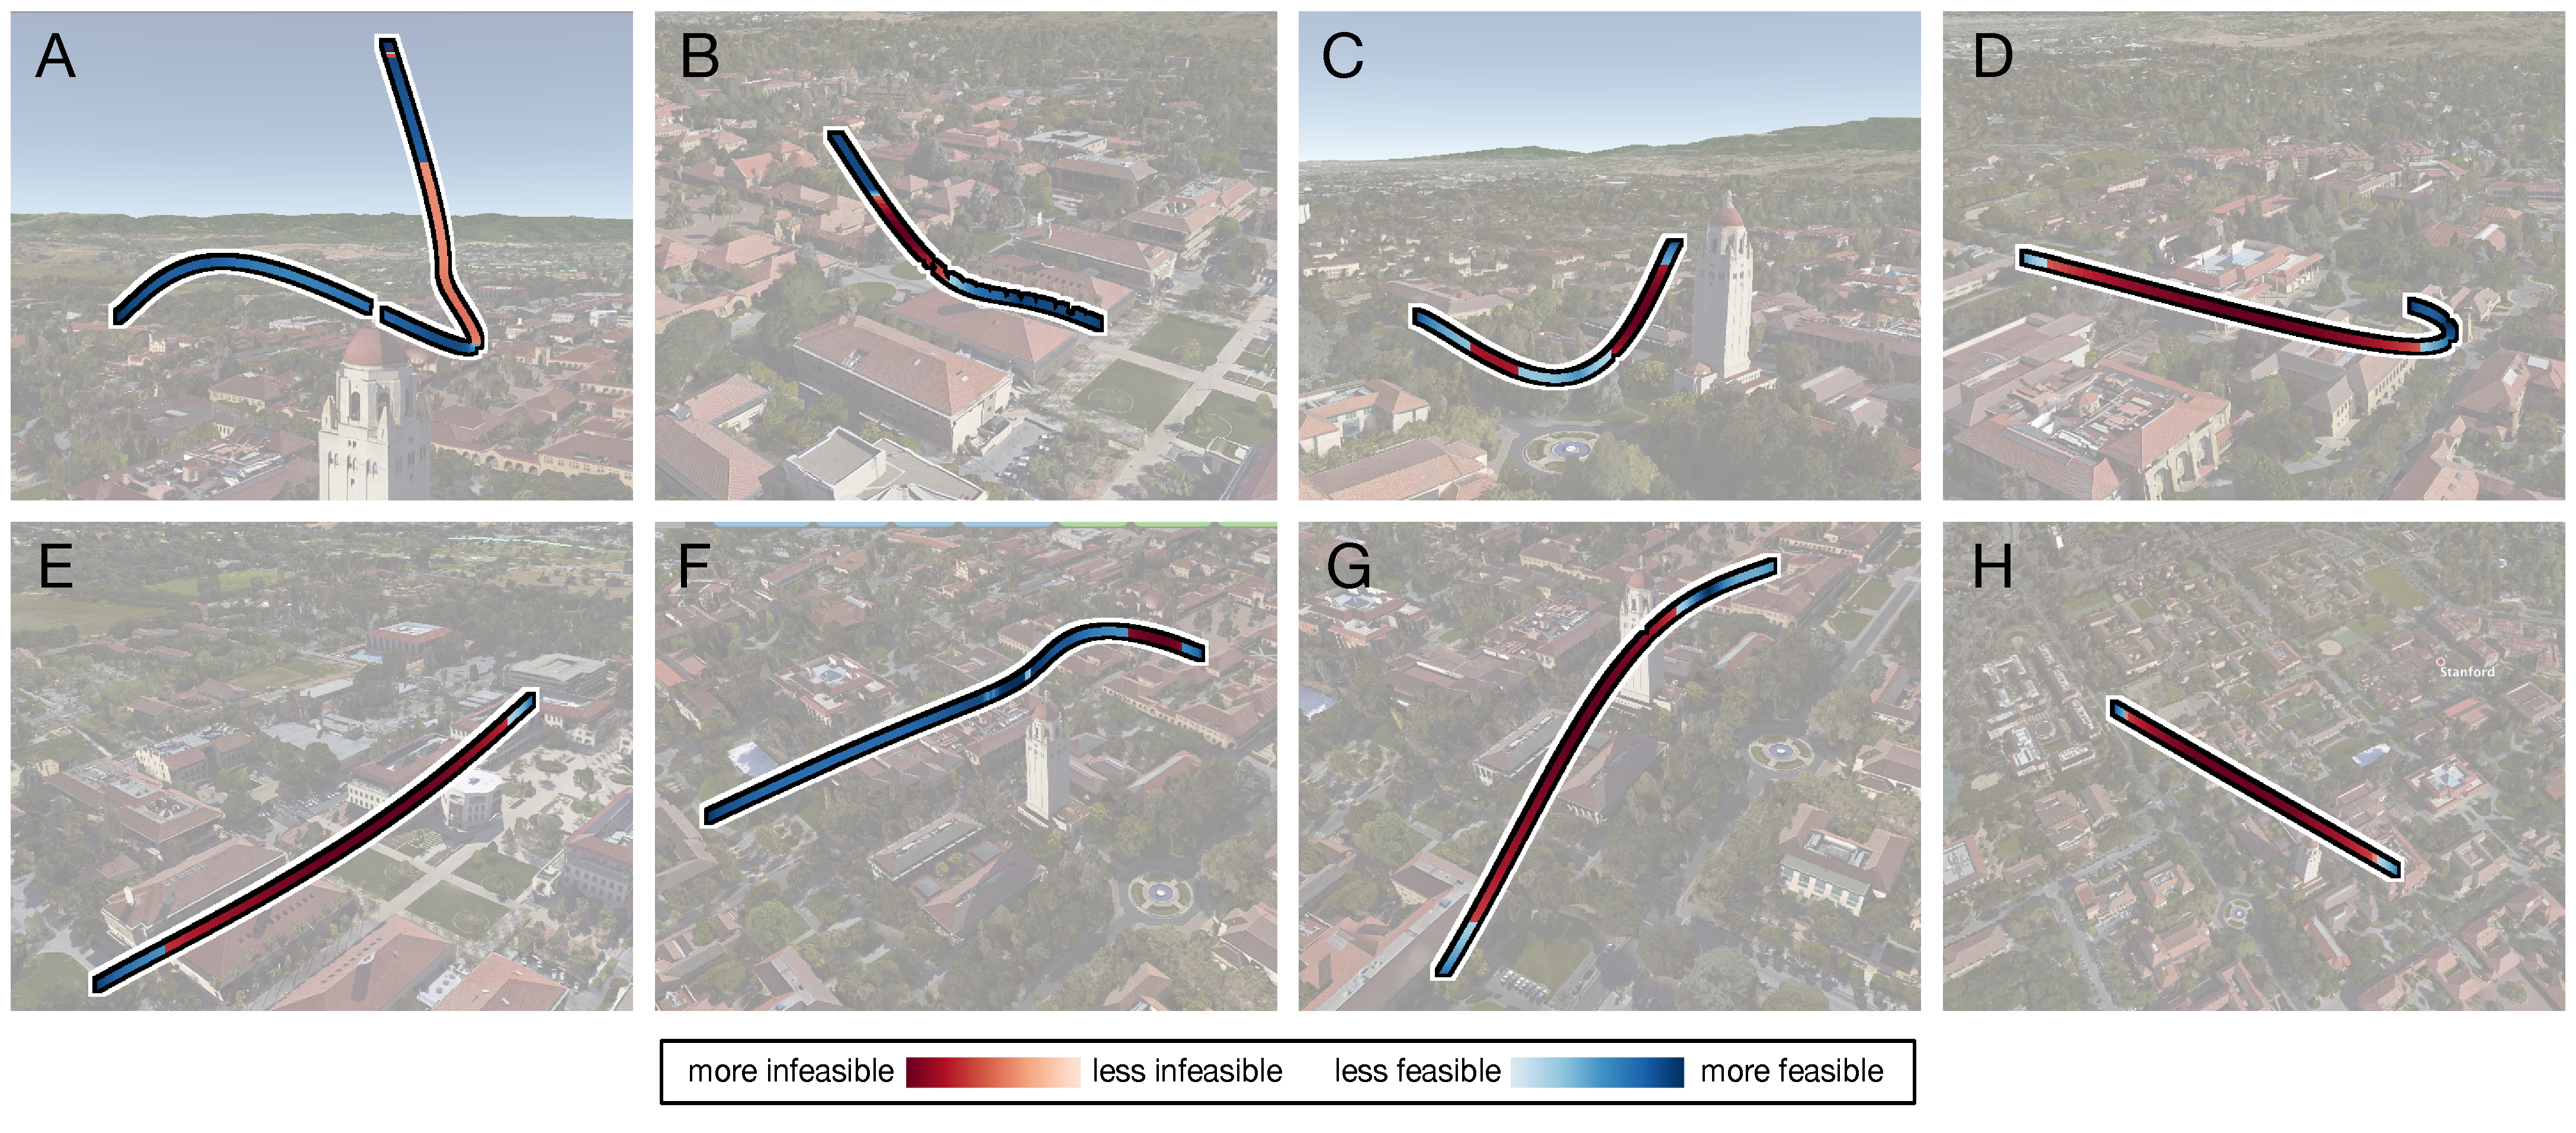
\includegraphics[width=6.0in]{images/2016_siggraph/03_dataset_24.pdf}
\caption{
Our dataset of infeasible quadrotor camera trajectories.
We show the trajectories in their spatial context, and color them according to how severely they violate our quadrotor's physical limits.
%Blue indicates regions of the trajectory that do not violate any constraints, and red indicates regions that violate at least one constraint.
%Deeper blue indicates regions that are further away from constraint boundaries, whereas deeper red indicates regions that more severely violate the constraints.
We use the letters in this figure to refer to individual trajectories throughout the paper.
}
\label{fig:ch3:dataset}
\end{figure*}

We based our dataset of infeasible quadrotor camera trajectories on raw data from the user study described in Chapter~\ref{sec:ch2}.
In this study, participants were tasked with creating cinematically interesting shots using \textsc{Horus}, an open source tool for quadrotor camera shot planning.
This study included 2 expert cinematographers, and 2 novice cinematographers with computer graphics experience.

\textsc{Horus} notifies users when their shots are infeasible, but requires users to manually edit their shots to make them feasible.
All of the shots from the previous study were infeasible at some point during the user's editing session.

\textsc{Horus} saves the complete revision history of a shot as it is being edited.
To compile our dataset, we simply found an infeasible revision for each shot in this previous study.
For the purpose of data collection, we assumed that revisions closer to the end of an editing session were more faithful to the user's artistic intent.
Therefore, as we compiled our dataset, we preferred revisions that were closer to end of an editing session. 
From this data collection procedure, we obtained 8 infeasible shots.
The feasibility violations in these shots ranged from moderate (e.g., briefly violating velocity limits by less than 10\%) to pronounced (e.g., violating velocity or control force limits by more than 50\% for sustained periods). 
We show the infeasible trajectories in our dataset in Figure~\ref{fig:ch3:dataset}.

\paragraph{Computational Performance}

To evaluate computational performance, we compared the running times of our algorithm and spacetime constraints on our dataset of infeasible trajectories.
We show the results from these experiments in Figure~\ref{fig:ch3:computation}.
%We describe the exact spacetime constraints problem formulation we use in our experiments in Appendix \ref{app:spacetime}.

In the interest of making fair comparisons, we took care to structure the implementations of our algorithm and spacetime constraints as similarly as possible.
The following implementation details apply to both implementations.
We solve the non-convex optimization problems arising in both approaches using the commercially available solver SNOPT~\cite{gill:2002}.
We initialize both approaches using the initialization strategy described in Section~\ref{sec:ch3:optimization}.
We call SNOPT using a Python wrapper provided by the authors, and we use all the default SNOPT error tolerances and parameters in all our experiments.
We express our objective function and constraint functions symbolically using the open-source symbolic algebra library SymPy~\cite{sympy:2014}.
We use SymPy to automatically generate all necessary gradient expressions. Finally, we use SymPy to generate efficient C code, which we call from Python, to evaluate the objective function, all constraint functions, and all necessary gradients.
We perform all our experiments on a Late 2013 Macbook Pro with a 2.6 GHz Intel Core i7 processor and 16GB of memory.

\paragraph{Convergence Behavior}

\begin{figure*}[t]
\centering
\includegraphics[width=6.0in]{images/2016_siggraph/00_computational_performance.pdf}
\caption{
Computational performance and scaling behavior of our algorithm on our dataset of infeasible trajectories.
When we solve for trajectories discretized at a moderate resolution of 100 time samples, our algorithm runs in less than 2 seconds, and is between 25$\times$ and 45$\times$ faster than spacetime constraints (a and b).
As we scale to more finely discretized trajectories, this performance gap widens, with our algorithm outperforming spacetime constraints by between 90$\times$ and 180$\times$ (c and d).
We indicate trajectories where spacetime constraints failed to find a solution with a $\star$.
We show the scaling behavior of our algorithm and spacetime constraints for trajectory \textsc{D}, which is the trajectory where spacetime constraints performed the best (e).
When scaling beyond 200 time samples, spacetime constraints did not consistently find a feasible solution for trajectory \textsc{D}.
We indicate where spacetime constraints successfully found a solution for trajectory \textsc{D} with colored dots.
%We take care to initialize our algorithm and spacetime constraints identically, using the initialization strategy described in Section \ref{sec:initialization}.
As a baseline, we include timing results for the modification of our algorithm described in Section~\ref{sec:ch3:results}.
On plots a, c, and e, lower is better.
}
\label{fig:ch3:computation}
\end{figure*}

\begin{figure}[t]
\centering
\includegraphics[width=4.0in]{images/2016_siggraph/01_convergence.pdf}
\caption{
Convergence behavior of our algorithm on trajectory \textsc{B} from our dataset of infeasible trajectories, discretized into 100 time samples.
This is the trajectory where spacetime constraints converged the fastest.
%We run SNOPT to convergence, using all the default SNOPT error tolerances and parameters. We indicate convergence with large colored dots.
Our algorithm, the modification of our algorithm described in Section~\ref{sec:ch3:results}, and spacetime constraints all converge rapidly to an optimal objective value (a).
However, because the equality constraints in our formulation are nearly linear, our algorithm converges to a solution that satisfies the equality constraints much faster than spacetime constraints (b).
We measure equality constraint error by summing the $l_2$ norm of each vector-valued equality constraint function, which is zero when the equality constraint is satisfied exactly. 
The y axes on these plots use a log scale.
Lower is better.
}
\label{fig:ch3:convergence}
\end{figure}

To evaluate the convergence behavior of our algorithm, we examined how the objective value in our optimization problem decreases as SNOPT makes progress towards an optimal solution for a trajectory in our dataset.
Similarly, we examined how the equality constraint functions, which are zero when the equality constraints are satisfied exactly, decrease as SNOPT makes progress.
Again, in all our experiments, we call SNOPT using all the default error tolerances and parameters.
We show the results from these experiments in Figure~\ref{fig:ch3:convergence}.

\paragraph{Accuracy}

\begin{figure}[t!]
\centering
\includegraphics[width=4.0in]{images/2016_siggraph/02_accuracy.pdf}
\caption{
Accuracy of our algorithm in predicting the results of a rigid body physics simulation.
We simulate the control trajectory produced by our algorithm using a \nth{5} order accurate rigid body simulator, and we measure how well the results of the simulation match the state space trajectory produced by our algorithm (a).
We repeat this experiment using the modification of our algorithm described in Section~\ref{sec:ch3:results} (b), spacetime constraints (c), and the original infeasible input trajectory simulated without control limits (d).
We plot the results for trajectory \textsc{G} in our dataset of infeasible trajectories, which was the trajectory where our algorithm performed the worst.
We provide mean error ($\mu$) and standard deviation ($\sigma$) values above each plot.
Even for this worst-case trajectory, our algorithm is more accurate than spacetime constraints, with slightly lower mean error.
For this particular trajectory, our unmodified algorithm is also slightly more accurate than our modified algorithm.
Having more histogram mass further to the left is better.
}
\label{fig:ch3:accuracy}
\end{figure}

To evaluate accuracy, we conducted an experiment using the state space and control trajectories produced by our algorithm.
%Our algorithm uses these state space and control trajectories to determine if the user's input camera trajectory has been slowed down enough to become feasible.
%Therefore, it is important that our algorithm produces accurate state space and control trajectories.
We simulated the control trajectories using a \nth{5} order accurate rigid body physics simulator, and we measured how well the results of the simulation matched the state space trajectories produced by our algorithm.
We repeated this experiment with spacetime constraints, the modified version of our algorithm, and the original infeasible input trajectory simulated without control force limits.
We show results from these experiments in Figure~\ref{fig:ch3:accuracy}.
Due to the relatively large time steps involved in these simulations, we applied LQR feedback control~\cite{tedrake:2016} in order to prevent the simulations from diverging.
We used identical LQR parameters in all our experiments.
We do not allow the LQR feedback controller to exceed the quadrotor's control force limits, except when simulating the infeasible input trajectories.

%To recover state space and control control trajectories from a speed profile produced by our algorithm, we simply evaluate the inequality constraint functions, $\mathbf{g}_\mathbf{x}$ and $\mathbf{g}_\mathbf{u}$, across the speed profile.
%We associate specific points along the speed profile with specific time values using the timing function computed in Section \ref{sec:optimization}.
%We recover state space and control trajectories for the original infeasible input trajectory using the algorithm presented in Section \ref{sec:control}.
%Spacetime constraints solves for state space and control trajectories explicitly, so no recovery procedure is needed to obtain these trajectories from spacetime constraints.

\paragraph{Dimensionality}

At each time sample, spacetime constraints requires at least 6 scalar decision variables for the configuration of the quadrotor, and 4 scalar decision variables for the quadrotor control forces.
In contrast, our formulation requires 5 scalar decision variables at each time sample.
Both formulations lead to the same block bi-diagonal structure in the constraint Jacobian.
Therefore, compared to spacetime constraints, our formulation reduces the required number of decision variables by at least 50\%, while preserving the efficient sparsity pattern in the constraint Jacobian.

\paragraph{Limitations}

By design, our algorithm will make an input trajectory feasible by perturbing its timing, but will not modify its spatial layout.
Therefore, our algorithm is not directly applicable in scenarios where the precise timing of the trajectory must be maintained.
In these scenarios, a spacetime constraints approach would be more appropriate.
That being said, we believe there is a broad class of usage scenarios in cinematography, journalism, and architecture, where re-timing an infeasible trajectory is reasonable behavior.
Therefore, we do not believe this limitation is overly burdensome.

